%====================================================
%
% Author: PR. XAVIER NOUMBISSI NOUNDOU
%
%====================================================
\documentclass[12pt, a4paper]{article}
\NeedsTeXFormat{LaTeX2e}

%---------------------------- PACKAGE INCLUSION -------------------------------
% This group renders characters clearer and more precise

\RequirePackage[bitstream-charter,cal,expert]{mathdesign}
\RequirePackage{latexsym}

\usepackage{geometry}
\geometry{a4paper,
		  %showframe=true,
		  %margin=2.75em,
		  %a4paper,
		  %total={170mm,257mm},
		  top=3.5em,
		  left=3em,
		  right=3em,
		  bottom=3.39em
		  }

\usepackage[default]{cantarell}
\usepackage{graphicx}
\usepackage{xspace}
\usepackage[parfill]{parskip} % Activate to begin paragraphs with an empty line rather than an indent
\usepackage{paralist} % very flexible & customisable lists (eg. enumerate/itemize, etc.)
\usepackage{listings} % for lstset definitions
\usepackage{url}
\usepackage{subfig} % make it possible to include more than one captioned figure/table in a single float
\usepackage{epsfig}
\usepackage{booktabs}
%\usepackage{enumitem} %funny itemize icons
\usepackage{verbatim}
\usepackage{tcolorbox}

\usepackage{pagecolor}

\usepackage{amsmath}
\newcommand{\mathbold}[1]{\text{\textbf{#1}}}

\usepackage{xcolor}
\definecolor{yerothColorOrange}{RGB}{242, 161, 0}   
\definecolor{yerothColorBlue}{RGB}{77 , 93 , 254}
\definecolor{yerothColorRed}{RGB}{254, 48 , 48}
\definecolor{yerothColorGray}{RGB}{198, 198, 198}
\definecolor{yerothColorDarkgray}{RGB}{60, 60 , 60}
\definecolor{yerothColorIndigo}{RGB}{83, 0, 125}
\definecolor{yerothColorGreen}{RGB}{2  , 160, 70}
\definecolor{forestgreen}{RGB}{2,160,70}    
\definecolor{mediumblue}{RGB}{7,43,205}    
\definecolor{firebrickred}{RGB}{178,34,34}
\definecolor{listingray}{gray}{0.9}
\definecolor{lbcolor}{rgb}{0.9,0.9,0.9}
\definecolor{darkgreen}{rgb}{0,0.35,0}
\definecolor{medgreen}{rgb}{0,0.5,0}
\definecolor{lightgreen}{rgb}{0.5,0.7,0.5}
\definecolor{pmcolour}{rgb}{0.5,0.7,0.5}
\definecolor{medgrey}{rgb}{0.6,0.6,0.6}
\definecolor{purplish}{rgb}{0.4,0,0.6}
\definecolor{brightred}{rgb}{1,0.2,0.2}

\newcommand{\diplinfn}{DR.\xspace}

\newcommand{\logicielpgi}{Progiciel de Gestion Intégré\xspace}

\newcommand{\yerothrd}{\textcolor{yerothColorGreen}
			{\textsc{\textcolor{yerothColorRed}{YEROTH}}$_{\text{r\&d}}$\xspace}}

\newcommand{\yerothpgiblack}{\texttt{YEROTH--PGI--$3.0$}\xspace}

\newcommand{\yerothpgi}{\textcolor{yerothColorBlue}{\sc YEROTH--PGI--$3.0$}\xspace}

\newcommand{\saperp}{SAP Business One\xspace}

\newcommand{\sageerp}{Sage Gescom i$7$\xspace}

\newcommand{\yerothtableur}{\texttt{TABLEUR}\xspace}

\newcommand{\myfullacademicname}{PR. XAVIER NOUMBISSI NOUNDOU\xspace}

\usepackage{hyperref}
\hypersetup{
    colorlinks,
	pagebackref,
    citecolor=medgreen,
    linkcolor=purplish,
    breaklinks,
    pdftex,
    bookmarks,
    plainpages=false,
	pdftitle={Comparaisons \yerothpgiblack, et autres solutions de gestion de stocks,
	 		   \'edit\'e, par: ''\myfullacademicname''},
    pdfauthor={PR. XAVIER NOUMBISSI NOUNDOU}
}

%--------------------------------------------------------------------------------

%---------------------------- COMMANDS DEFINITION -------------------------------
\newcommand{\diplinf}{\emph{DR.}\xspace}

\newcommand{\emphbf}[1]{\textbf{#1}\xspace}
\newcommand{\emphit}[1]{\emph{\textit{#1}}\xspace}
\newcommand{\mycheckmark}[1]{\textcolor{#1}{$\checkmark$}\xspace}
\newcommand{\mytimes}[1]{\textcolor{#1}{$\times$}\xspace}
\newcommand{\boldsc}[1]{\textbf{\textsc{#1}}\xspace}

\newcommand{\myenumitem}[1]{\emph{#1}\xspace}
\newcommand{\yerothalert}{\emph{yeroth-erp-3-0-system-daemon}\xspace}

\newcommand{\mysql}{MySQL\xspace}
\newcommand{\mysqlcolored}{\textcolor{yerothColorBlue}{My}\textcolor{yerothColorOrange}{SQL}\xspace}

\newcommand{\role}{r\^ole\xspace}
\newcommand{\roles}{r\^oles\xspace}

\newcommand{\manager}{<< Manager >>\xspace}
\newcommand{\magasinier}{<< Magasinier >>\xspace}
\newcommand{\caissier}{<< Caissier >>\xspace}
\newcommand{\administrateur}{<< Administrateur >>\xspace}
\newcommand{\vendeur}{<< Vendeur >>\xspace}
\newcommand{\gestionairedestocks}{<< GestionaireDesStocks >>\xspace}

\newcommand{\qt}{Qt$5$\xspace}

\newcommand{\yerothfield}[1]{\textbf{\emph{#1}}\xspace}
\newcommand{\procparagraph}[1]
	{\paragraph{ \mycheckmark{forestgreen} \emph{\textcolor{forestgreen}{#1}}}}


\newcommand{\yerothvert}[1]{\textcolor{yerothColorGreen}{#1}\xspace}
\newcommand{\yerothorange}[1]{\textcolor{yerothColorOrange}{#1}\xspace}
\newcommand{\yerothrouge}[1]{\textcolor{yerothColorRed}{#1}\xspace}

\newcommand{\yerothevident}{\yerothvert{\'evidente}\xspace}
\newcommand{\yerothcompliquee}{\yerothorange{compliqu\'ee}\xspace}
\newcommand{\yerothtrescompliquee}{\yerothrouge{tr\`es compliqu\'ee}\xspace}



\newcommand{\featuresummary}[2]{\textbf{\textcolor{#1}{\textsc{#2}}}}

%--------------------------------------------------------------------------------

\usepackage[T1]{fontenc}
\newcommand{\changefont}[3]{
\fontfamily{#1} \fontseries{#2} \fontshape{#3} \selectfont}
\changefont{cmss}{m}{n}

% Set font to avant-garde
%\renewcommand*\rmdefault{pag}

\usepackage[french]{babel}
\addto\captionsfrench{\def\tablename{Tableau}}

\usepackage{fancyhdr}
\pagestyle{fancy}
\renewcommand{\headrulewidth}{0pt}
\rhead{}
\lhead{}
\lfoot{{\small Auteur: \myfullacademicname}}
\rfoot{{\small version du --~$3$~Mai~$2021$~--}}
\cfoot{}

%Remove widows and orphants
\clubpenalty = 10000
\widowpenalty = 10000
\displaywidowpenalty = 10000

\setcounter{subsection}{0}

\renewcommand{\thesubsection}{\arabic{subsection}}

\renewcommand\labelenumi{\theenumi)}

\pagenumbering{gobble}

\begin{document}

{\bf \Large \yerothrd} {| \sc \scriptsize Comparaisons \yerothpgiblack, et autres solutions de gestion de stocks}			
\\ \line(1,0){540}

\vspace{1.15em}


\parbox{27em}{\Large Avantages D'utilisation de L'informatique Pour
					La Gestion De Stocks}

\vspace{3.3em}

\begin{table}[!htbp]
\begin{tabular}{ll}
\parbox{27em}{
\yerothpgi est un \logicielpgi (PGI) avantageux par rapport
aux autres méthodes de gestion de stocks à cause des raisons suivantes:

\begin{enumerate}[1.]
	\itemsep -0.1em
	\item progiciel de gestion intégré, réseau compris
	\item utilisation de \mysql comme moteur de base de données. \\
\end{enumerate}
}

&

\parbox{15em}{
\begin{center}
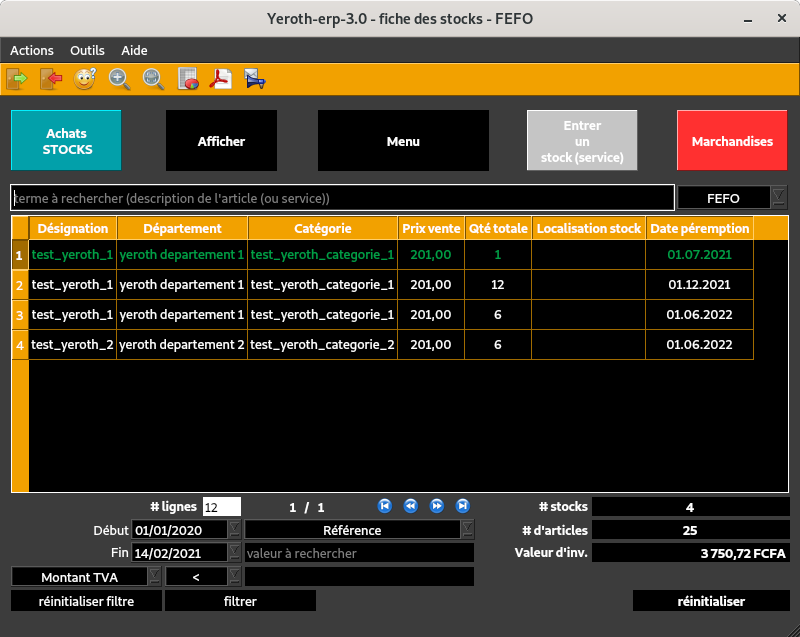
\includegraphics[scale=0.25]{images/yeroth-fenetre-stocks.png}
\caption*{La fiche des stocks (SOLUTION INFORMATISÉE 'YEROTH--PGI--3.0')}
\end{center}
}
\end{tabular}
\end{table}


\subsection{1 LARGE DIMENSION GÉOGRAPHIQUE}

\subsection{1 LARGE DIMENSION GÉOGRAPHIQUE}

\subsection{1 LARGE DIMENSION GÉOGRAPHIQUE}

\subsection{1 LARGE DIMENSION GÉOGRAPHIQUE}


\vspace{1cm}

Le tableau~\ref{tab:comparaison-yerotherptroiszero-autres-solutions-de-gestions-de-stocks}
illustre la complexité d'assumer efficacement des tâches
de gestion de stocks \textbf{SANS OUTILS INFORMATIQUE}.\\

\vspace{-1em}

\begin{table}[!htbp]
\selectlanguage{french}
\centering
\resizebox{\textwidth}{!}{%to fit the table within the text width
\begin{tabular}{lccc}

\multicolumn{1}{c}{}	&
SANS INFORMATIQUE		& 
\yerothtableur			&
\yerothpgiblack			\\ \hline

\textbf{$1$. (large dimension géographique de l'organisation)}&
		\yerothrouge{extrênement difficile}					&
		\yerothrouge{extrênement difficile}					&
		\yerothvert{facile}					   	   \\  \hline 	
		
\textbf{$1$. (nombre de succursales élevé)}		&
		\yerothrouge{extrênement difficile}		&
		\yerothrouge{extrênement difficile}		&						
		\yerothvert{facile}	\\ \hline
	
\textbf{$1$.; $2$. (quantité totale élevée d'articles à vendre, transférer)}&
		\yerothrouge{extrênement difficile}				&
		\yerothorange{très difficile}					&						
		\yerothvert{facile}						\\ \hline
				
\textbf{$2$. (travail simultané et coordoné sur les données)}	&
		\yerothrouge{extrênement difficile}						&
		\yerothorange{très difficile}							&						
		\yerothvert{facile}				   					   \\
\end{tabular}}
\caption{Comparaison entre \yerothpgi et les autres solutions de gestion de stocks\\}
\label{tab:comparaison-yerotherptroiszero-autres-solutions-de-gestions-de-stocks}
\end{table}

\paragraph{CONCLUSION:}

\yerothvert{PLUS L'ORGANISATION EST GRANDE EN ACTIVITÉS, ET EN
SUPERFICIE, PLUS IL EST EXTRÊNEMENT IMPORTANT DE FAIRE
USAGE D'1 PROGICIEL DE GESTION INTÉGRÉ (PGI) POUR 1 RENTABILITÉ
EFFICACE !}

\end{document}

